\section{Team Structure}
\label{sec:team}

As in the initial report, we use the following acronyms for team members:

\begin{tabular}{ p{3cm} p{4cm} p{3.5cm} p{3.5cm} }
  \textbf{AJF}-Adam Fahie &
  \textbf{AIF}-Andrew Fairbairn &
  \textbf{TF}-Anthony Free &
  \textbf{TD}-Tom Davies \\
    \textbf{RT}-Rosy Tucker &
  \textbf{JM}-Joseph Mansfield &
  \textbf{MW}-Michael Walker \\
\end{tabular}

Before beginning this stage of the project, we ascertained which university modules team members were studying, in order to spread the work load evenly and reduce the risk of team members' under performance due to other commitments. We also assessed the strengths and weaknesses of each team member, aiding in the selection of technologies and task assignment, as shown in table \ref{tab:skills}. Table \ref{tab:skills} shows that all team members are proficient with Java, and thus it was a natural implementation choice for the prototype.

All team members contributed to the design of the HUMS architecture, however, when implementing the prototype the team divided into three sub-teams, each assigned to different modules and requirements for the system.
The sub-teams were organised such that team members with similar skills and knowledge were placed together, encouraging low coupling and rapid development of individual modules, without worrying about the state of the overall system. The tasks assigned to each sub-team are shown below, reporting and notification engines were not assigned to any particular sub-team, meaning all team members were able to contribute to designs, encouraging creativity. The roles of each team member, revised from the initial report due to this new structure, are shown in table \ref{tab:roles}. A member of each sub-team has taken on a quality assurance and design role, ensuring a high quality of work from all team members.

\begin{description}
  \item[Team Sense  (JM and MW)] Create a data emitter for the test application, by producing reusable monitoring components.and implement the data input API as a multithreaded server, in order to meet requirements  regarding simultaneous usage.
    
  \item[Team Store  (TD and RT)] Implement the database abstraction layer, and provide a concrete implementation using Google App Engine as a backing store, keeping the API generic in order to meet requirements regarding flexibility of database implementation.

  \item[Team Analyse (AJF, AIF, and TF)] Implement the analysis controller and the analysis engine API. The engine API was implemented to be very sparse so that a large number of different concrete implementations could be supplied. 
\end{description}

\begin{table}[H]
\centering
\begin{tabular}{|p{1.2cm}|p{8cm}|p{5cm}|}
  \hline \rowcolor{titleColor}\textbf{Initials} &
  \textbf{Experience} &
  \textbf{Weaknesses}\\

  \hline AJF
  & Java, C, Ruby, Spring, Hibernate, Gradle, Design Patterns, Tomcat, JBoss,
  Git, SQL
  & Web Development, NoSQL, UI/UX, Technical Writing \\

  \hline AIF
  & Java, C++, Python, Javascript, PHP, UI/UX, Web Development, NoSQL/SQL
  & Spring, Technical Writing \\
  
  \hline TF
  & PHP, Javascript, Java, VB, C, Linux, MDE Developer, Git, SQL
  & UI/UX, Technical Writing \\

  \hline TD
  & Java, C, Python, Scala, Android, Swing, Machine Learning, SQL
  & NoSQL, Web Development, Git \\

  \hline JM
  & C, C++, Java, Python, UI/UX, Android, Web Development, Git, SQL
  & Hardware, NoSQL \\

  \hline RT
  & Java, C, Objective-C, Javascript, Android, iOS, Swing, Design Patterns,
  Google AppEngine, HCI, NoSQL/SQL, Attribute Driven Design
  & Spring, Git \\

  \hline MW
  & C, Java, Python, Git
  & UI/UX, Technical Writing, Concurrency \\
  \hline
\end{tabular}
\caption{The identified strengths and weaknesses of team members}
\label{tab:skills}
\end{table}

\begin{table}
\begin{tabular}[H]{ | p{3.5cm} | p{8.5cm} | p{2cm} |}
\hline
\rowcolor{titleColor}\textbf{Role}
&  \textbf{Description} 
& \textbf{Assignees} \\ \hline

Product Owner & Represent the interests of the customer, identifying key quality attributes & RT \\ \hline

Scrum Master  &   Ensuring Scrum process is followed by all team members, and ensuring good inter-team communication.            		& RT           				\\ \hline
Editor  &   Review and format documentation. & JM,TD,RT \\ \hline

Software Architect  &  Ensures requirements are met, and software is consistent. & JM \\ \hline

Requirements Analyst  &   Identification of customer needs and requirements.  & Team \\ \hline

Developer &   Developing software to agreed standards. &  Team     \\ \hline

UX/UI Designer    &   Accessibility, UI/UX	& JM,RT,AIF    \\ \hline

Security    &   Advising on relevant security standards and protocols. & TF,MW  \\ \hline

Penetration Tester & Test HUMS for exploits and security weaknesses. &TF, MW \\ \hline

Software Tester &   Creating or assisting in the creation of tests. & Team  	 \\ \hline

Risk Manager &   Identify key risks and mitigation strategies though out the project .  & TF, AJF \\ \hline

Database Admin &   Design of database strategies and schemas. & RT, TD                   \\ \hline
Quality Assurance   &   Ensure cohesion between system modules, analysing performance and enforcing quality standards.  & JM, RT, AIF \\ \hline
\end{tabular}
\caption{The revised roles of team members}
\label{tab:roles}
\end{table}

\section{Development Plan}

As a team we considered the scope of the project which was to be undertaken. As a result of this we divided the work to be undertaken into specific tasks. Once the work to be undertaken was identified, the work was evenly split across the sub-teams.
Before beginning development the team, as a whole, updated and extended the previous Gantt chart based on customer feedback.
Figure \ref{fig:ganttInterim}  shows the plan for the interim phase of the project, beginning with reviewing feedback from the previous report.
Figure \ref{fig:ganttFinal}  shows the plan for the final phase of the project, and more specifically identifies areas of the prototype to be refined.

Dependencies between tasks were examined allowing for a critical path through the project to be identified, showing the longest path through the project and the earliest point at which individual tasks can be started.
This critical path analysis ensures that all work can be completed on time and that time is being used efficiently. 

\begin{figure}[ht!]
  \centering
  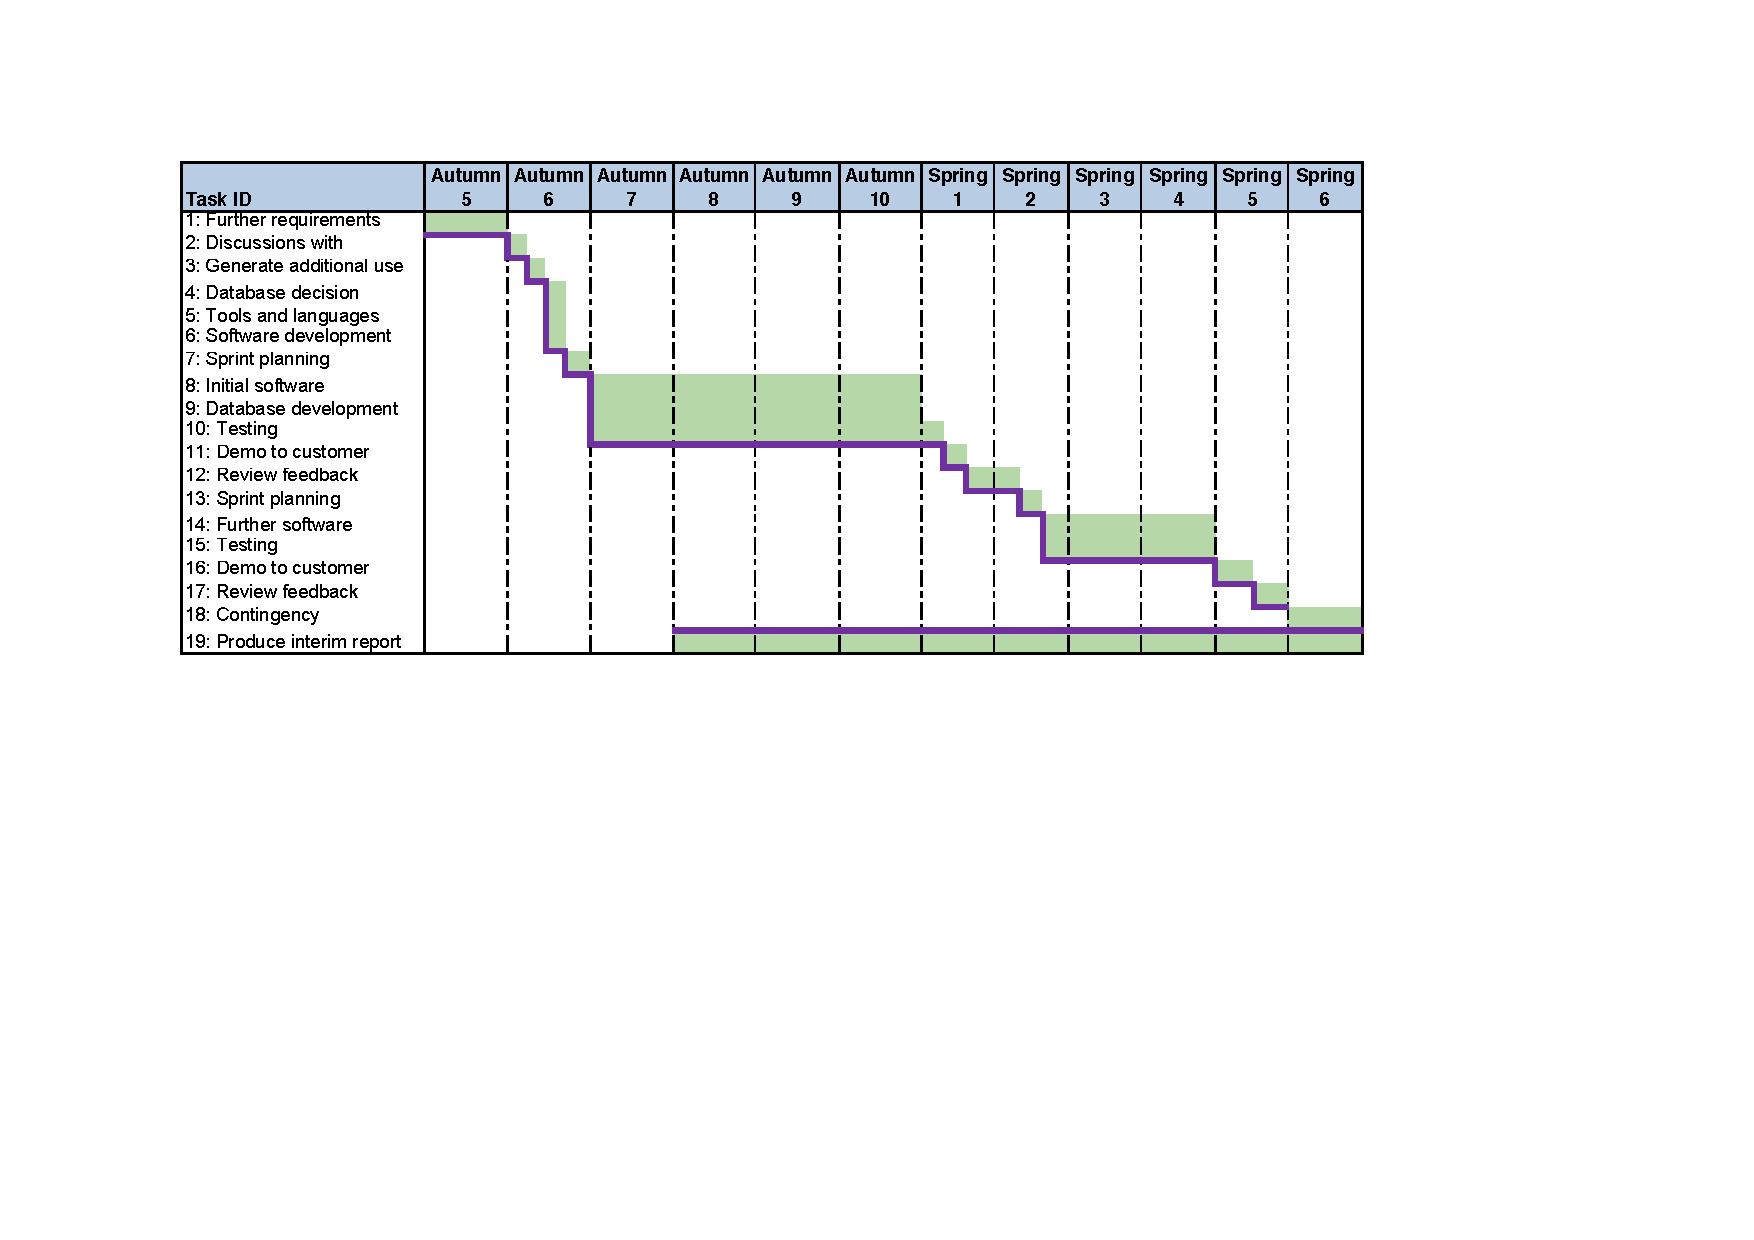
\includegraphics[width= 15cm]{images/GantInterim.pdf}
  \caption{Gantt chart for the interim phase of the project, purple shows the critical path.}
  \label{fig:ganttInterim}
\end{figure}

\begin{figure}[ht!]
  \centering
  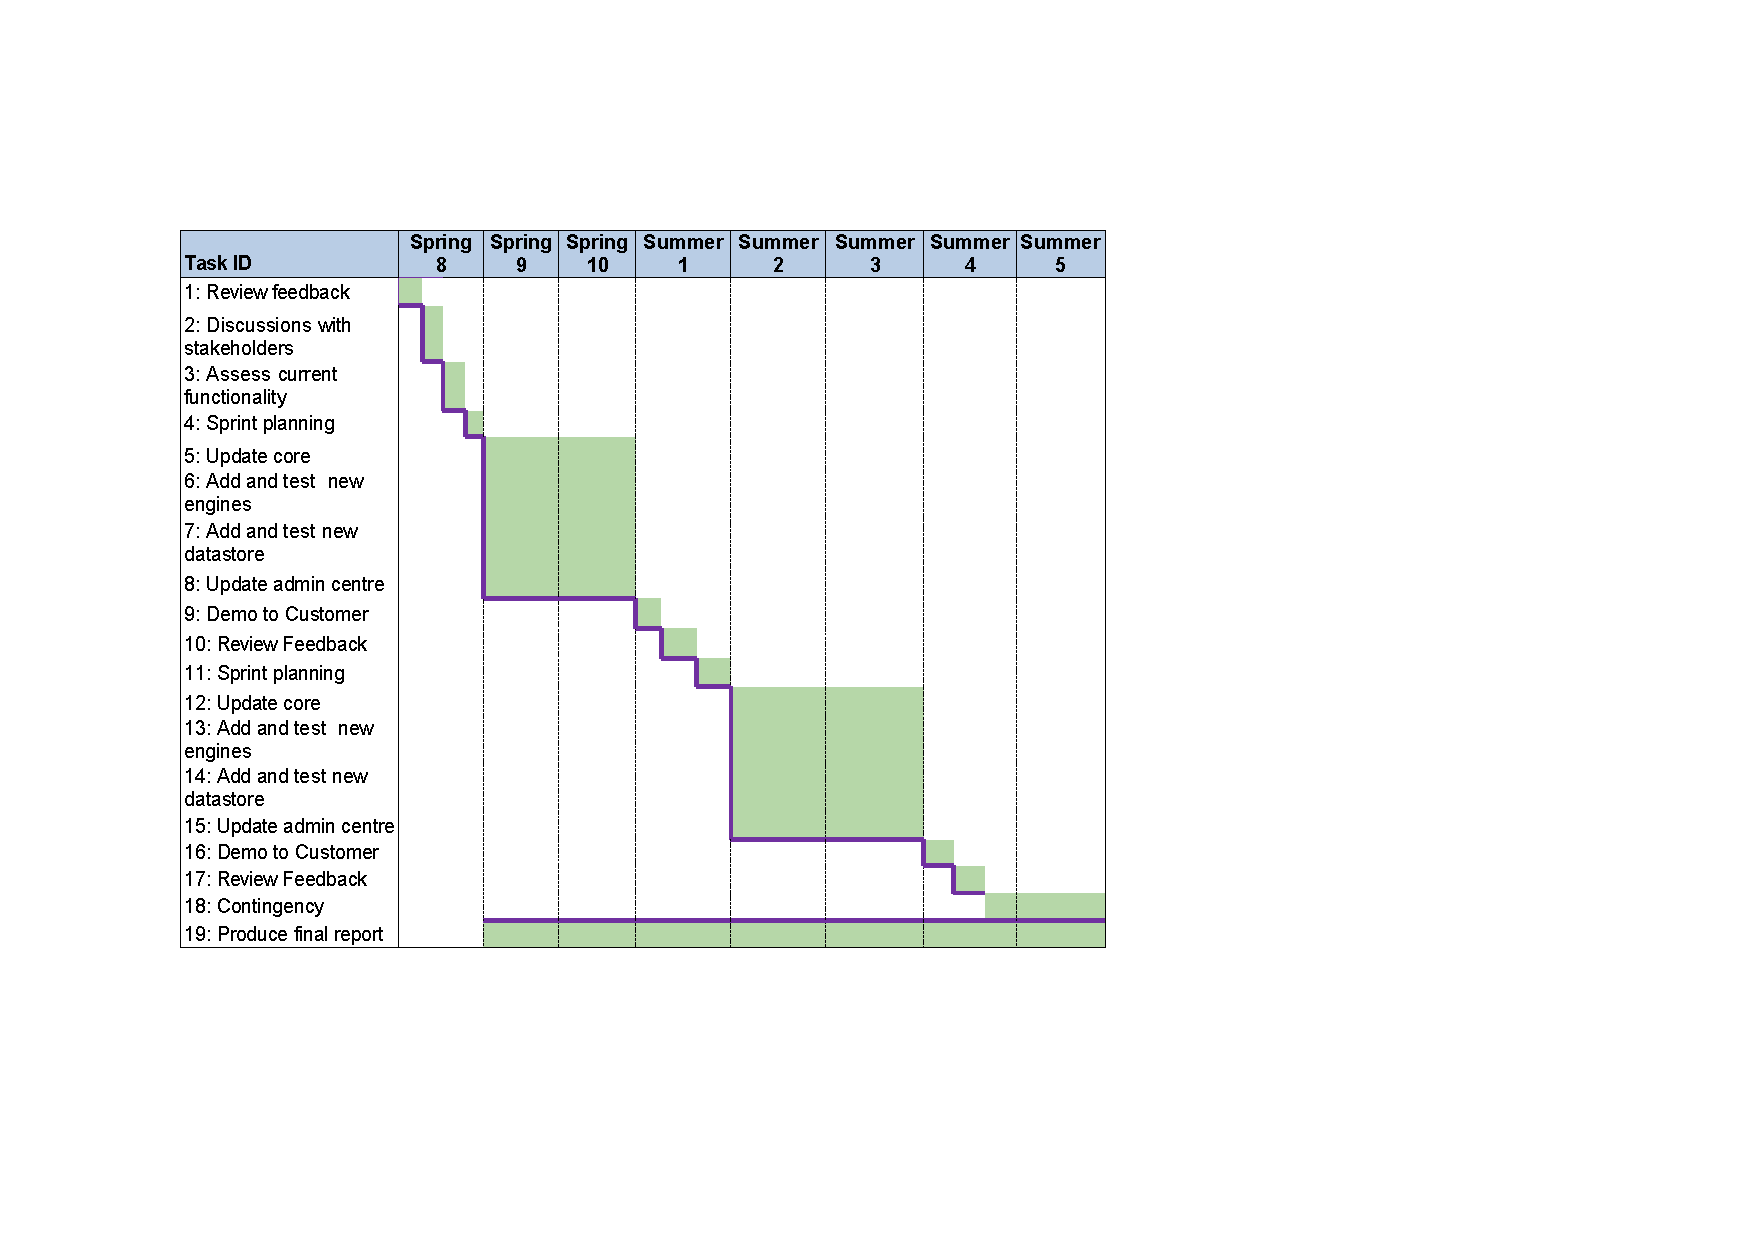
\includegraphics[width= 12cm]{images/GantFinal.pdf}
  \caption{Gantt chart for the final phase of the project, purple shows the critical path.}
  \label{fig:ganttFinal}
\end{figure}